% !TEX root = ../bachlor-arbeit.tex
\begin{tabular}{ll}
    \toprule
    Input: &
    \begin{tabular}[t]{@{}l@{}}
        transmission spectrum $I=(I_\s{x}, \,I_\s{y})$ a $\lambda \times 2$ array\\
        $I_\s{x/y}$...X- and Y-transmission spectra,
        $\lambda$...number of wavelengths
    \end{tabular}\\
    Output: &
    two sets layer parameters $\mc L_1$ and $\mc L_2$ \\
    \bottomrule
\end{tabular}

\paragraph{Network Architecture}
This module is a 1D Convolutional Neural Network instead of the simple Multi Layer Perceptron. It was chosen to utilize the translational invariance of ConvNets. For example the concept "peak" should be learned independent of its position in the spectrum. As described in section \ref{sec:NN_bg} a ConvNet provides this functionality. Another constraint on the network architecture arises from the different kind of outputs.
Most of the outputs are continuous but the choices about material $m$ and geometry $g$ are discrete/categorical.
These need different activation functions $\sigma$ to reach the different value ranges. The continuous outputs are mostly bounded by physical constraints and $m, \, g \in [0, \, 1]$ as they are \textit{one hot encoded} meaning $1 \rightarrow$ "The layer has this property" and
$0 \rightarrow$ "The layer does not have this property".


The different outputs also need different cost functions $C(y, y')$ during training where $y'$ is the networks output and $y$ is the known solution. For the continuous output one can simply use the mean squared error
\begin{equation}
    C_\s{mse}(\vb y, \, \vb y') = \sum_i \qty(y_i - y_i')^2
\end{equation}

\noindent
as all outputs are equally important and the cost function should be indifferent on whether the networks prediction is over or under target. For the categorical output the network learns quicker with the \textit{Categorical Cross-Entropy} error.

\begin{equation}
    C_\s{ce}(\vb y, \, \vb y') = - \sum_i y_i \log y'_i,
\end{equation}

\noindent
This error treats false positives and false negatives differently. A false positive does not increase the overall cost as $y_i = 0$ anyway but for a false negative ($y_i = 1, \, y_i' = 0$) $C_\s{ce} \rightarrow \infty$. This is wanted behavior because it does not matter if the network outputs some probability for a wrong class as long as it outputs a higher probability for the correct class. The final architecture is similar to the example given in figure \ref{fig:bg:NN_example} while meeting the above-mentioned constraints:

\begin{figure}[H]
    \centering
    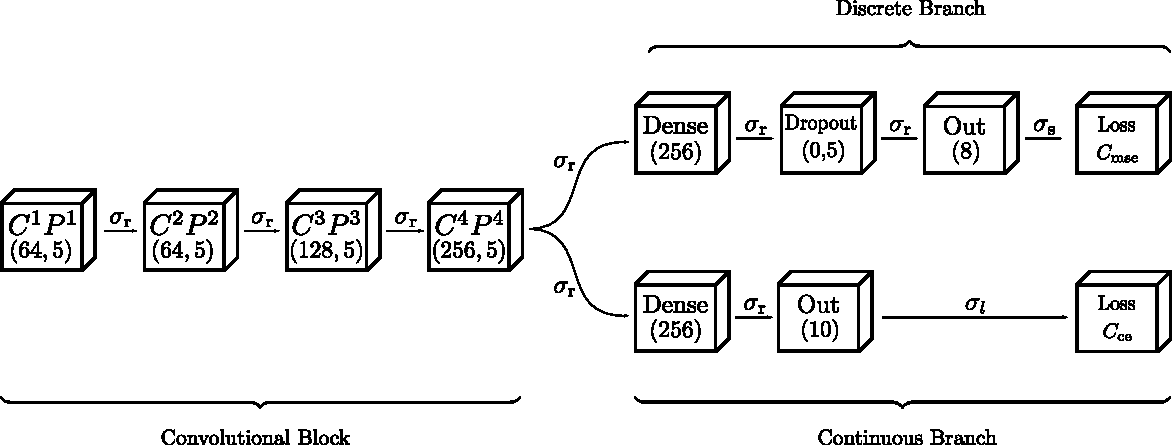
\includegraphics[width=\linewidth]{al_NN_architecture}
    \caption{The network starts with 4 pairs of convolutional and pooling layers. The convolutions are characterized by (\textit{number of kernels}, \textit{kernel size}). The kernel size is always 5 and the number of kernels is gradually increased. Then the Network splits into a discrete and a continuous branch via two Dense layers with (\textit{number of neurons}). In the discrete branch a dropout is applied to the dense layer where (0.5) is (\textit{fraction of neurons to drop}).
    All the internal activations $\sigma_\s{r}$ are ReLu's and the final activations $\sigma_\s{s}$ and $\sigma_{l}$ are a sigmoid and a linear function.}
    \label{fig:al:NN_architecture}
\end{figure}

\newpage
\paragraph{Network Training}
To train a Neural Network one needs a training set $(X, \, Y)$ of known input output pairs. In this case they are generated using the pre simulated single layers in the database which are randomly combined into a stacks. The single layers are simulated with the Fourier Modal Method (FMM). Then the stacks X- and Y-transmission spectra $(I_x, \, I_y)$ are calculated via SASA.
That means $(I_x, \, I_y) \in X$ are the networks input and the random parameters $(p_1, \, m_1, \, g_1, \, p_2, \, m_2, \, g_2) \in Y$ are the output. For the first geometry we used squares and square holes of Aluminium and Gold as seen in figure
Using this approach the following accuracy is reached:

\begin{figure}[H]
\centering
\begin{subfigure}{.6\textwidth}
    \centering
    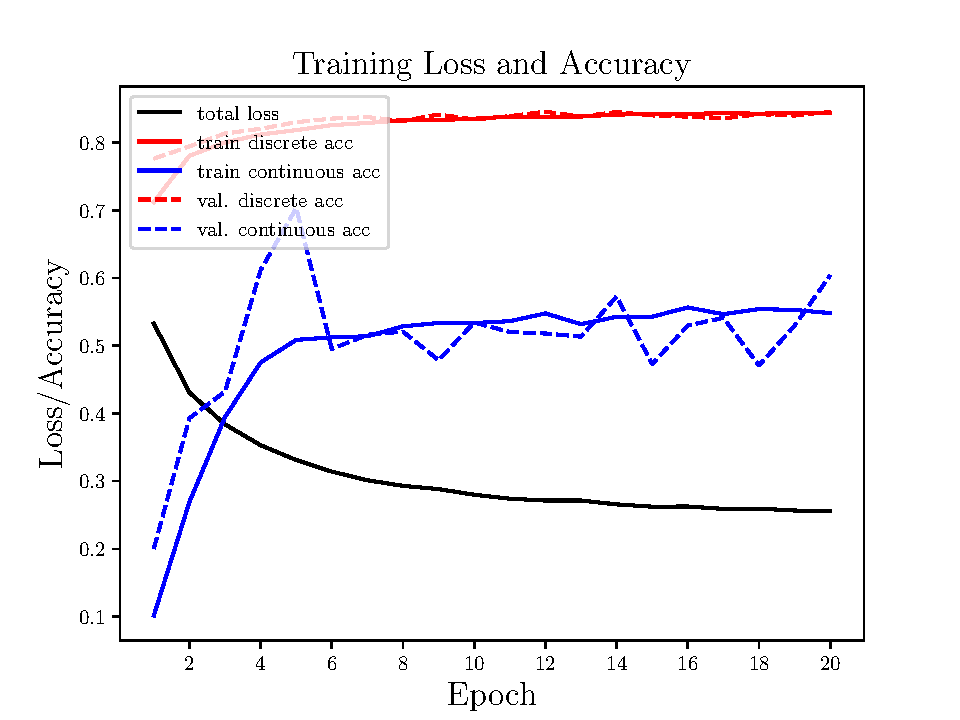
\includegraphics[width=\linewidth]{al_training_squares}
    \caption{}
    \label{}
\end{subfigure}%
\begin{subfigure}{.4\textwidth}
    \centering
    \includegraphics[width=.6\linewidth]{al_square}
    \caption{}
    \label{}
\end{subfigure}
\caption{Shown are the total loss and the training and validation accuracy for both the continuous and the discrete branch in figure (a). After each epoch the network is validated on data not used in training to check for overfitting. Figure (b) shows the used geometry of squares and square shaped holes of Aluminium and Gold. They have width $w$, length $l$ and thickness $t$. In the full layer these meta atoms are arranged periodically as seen in figure \ref{fig:bg:two_layers}.}
\label{}
\end{figure}


Training and validation accuracy are very similar which indicates that there is no overfitting. The discrete accuracy quickly reaches a maximum of $\sim 80\%$
which is less than expected for this classification problem. The issue here lies not within the networks architecture but in the data generation process. In section \ref{sec:SASA} we have shown that for this geometry the transmission spectrum is the same for both directions. That means the data generation can result in two different stacks which produce the same spectrum. Lets consider a stack where one layer is Aluminium and the other is Gold. As both of them produce the same spectrum one time the network is taught that the first layer is Gold and another time its taught the complete opposite. Actually if the network is trained this way it only ever predicts stacks with layers of equal materials because this is the only setup it can get right.
\\

\begin{figure}[H]
    \floatbox[{\capbeside\thisfloatsetup{capbesideposition={right,top},capbesidewidth=8cm}}]{figure}[\FBwidth]
    {\caption{A stack of one Gold and one Aluminium layer separated by a glass spacer. If the layers are made of meta atoms of the square geometry as seen in figure orientations produce the same spectrum which leads to issues when using completely random stacks to train the network.}
    \label{fig:test}}
    {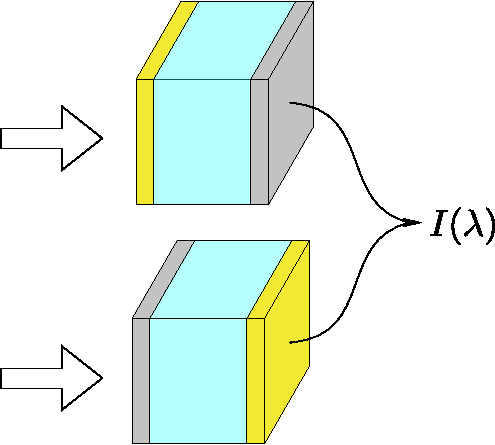
\includegraphics[width=.35\textwidth]{al_flipped_stack}}
\end{figure}


\newpage
This is well known problem that arises when training a network on a problem where there are many solutions to one given input.
\note{cite stuff}
We can prevent this issue simply by allowing only one of the equivalent orientations into the training data. This does not limit the capabilities of the trained network as the variety of input spectra stays the same.
